
% \documentclass{article}

% % Language setting
% % Replace `english' with e.g. `spanish' to change the document language
% \usepackage[english]{babel}

% % Set page size and margins
% % Replace `letterpaper' with `a4paper' for UK/EU standard size
% \usepackage[letterpaper,top=2cm,bottom=2cm,left=3cm,right=3cm,marginparwidth=1.75cm]{geometry}

% % Useful packages
% \usepackage{amsmath}
% \usepackage{graphicx}
% \usepackage[colorlinks=true, allcolors=blue]{hyperref}


\documentclass[11pt]{article}
\usepackage[hmargin=1in,vmargin=1in]{geometry}
\usepackage{xcolor}
\usepackage{amsmath,amssymb,amsfonts,url,sectsty,framed,tcolorbox,framed}
\newcommand{\pf}{{\bf Proof: }}
\newtheorem{theorem}{Theorem}
\newtheorem{lemma}{Lemma}
\newtheorem{proposition}{Proposition}
\newtheorem{definition}{Definition}
\newtheorem{remark}{Remark}
\newcommand{\qed}{\hfill \rule{2mm}{2mm}}


\begin{document}
%%%%%%%%%%%%%%%%%%%%%%%%%%%%%%%%%%%%%%%%%%%%%%%%%%%%%%%%%%%%%%%%%%%%%
\noindent
\rule{\textwidth}{1pt}
\begin{center}
{\bf [CS304] Introduction to Cryptography and Network Security}
\end{center}
Course Instructor: Dr. Dibyendu Roy \hfill Winter 2023-2024\\
Scribed by: Raghav Agiwal (202151124) \hfill Lecture (Week 1\))
\\
\rule{\textwidth}{1pt}
%%%%%%%%%%%%%%%%%%%%%%%%%%%%%%%%%%%%%%%%%%%%%%%%%%%%%%%%%%%
%write here

\section{Introduction to Cryptography}

\begin{itemize}
    \item \subsection{Cryptography:} 
Cryptography is the application and study of techniques to protect communications and information from third parties or competitors. Simply put, it involves creating and using codes or passwords to protect information and ensure that only authorized individuals can access or understand it. Cryptography plays an important role in protecting the confidentiality, integrity, and authenticity of information in various fields, such as online communications, financial transactions, and data storage. In simple words, it develops algorithms to get security.\\\\
    
    \item \subsection{Cryptanalysis:}
Cryptanalysis is the study and process of analyzing and decrypting ciphers, codes, and encrypted text without using actual keys. Alternatively, we can call it a process to access the text content of the communication when you do not have access to the decryption key.\\\\
    \item \subsection{Cryptology:}
Cryptology is a term that includes both cryptography and cryptanalysis.Cryptography involves the development of secure communication methods (cryptography) and the study of methods for breaking or cracking them (cryptanalysis). The general goal of cryptography is to design and analyze systems that will ensure the confidentiality, integrity, and authenticity of information in the presence of potential adversaries or in unauthorized situations.
\end{itemize}

\section{NIST}
NIST stands for National Institute of Standards and Technology, a U.S. government agency dedicated to developing and promoting standards and technologies to improve financial security and public safety. In the field of cryptography and network security, NIST plays a key role in the development and standardization of cryptographic algorithms and methods.

NIST is known for its contributions to the development of standards and procedures that help ensure cybersecurity in information systems. One of NIST's major contributions was the development of the Advanced Encryption Standard (AES), a widely used key encryption algorithm. AES has become the encryption standard for protecting sensitive data and is used in many applications and businesses.
\\\\
Encryption : E (P,K) = C\\
Decryption : D (C,K) = p
\\
\section{Keys in Cryptography}
\subsection{Public Key / Asymmetric Key} 
Asymmetric key encryption uses two keys: public key and private key. While the public key is shared publicly, the private key is kept secret. Anything encrypted with the public key can only be decrypted with the private key and vice versa. Asymmetric key encryption technology eliminates the need for both parties to share public keys in advance.

Examples of asymmetric key algorithms include RSA (Rivest-Shamir-Adleman), ECC (Elliptic Curve Cryptography) and DSA (Digital Signature Algorithm).

\subsection{Private-key / Symmetric Key}
Symmetric key encryption uses the same key for encryption and decryption. All parties involved in a secure communication must first share the key. This key is kept secret and is used to encrypt and decrypt data. The challenge of symmetric key encryption is to distribute and manage keys securely.

Examples of symmetric key algorithms include DES (Data Encryption Standard), AES (Advanced Encryption Standard), and 3DES (Triple DES).
\\
\begin{figure}
\centering
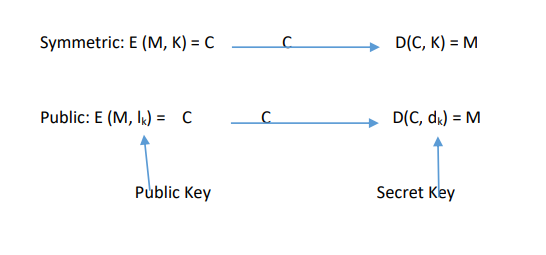
\includegraphics[width=0.8\linewidth]{image1.PNG}
\end{figure}

\section{Cryptography provides the following security services :}
\subsection{Confidentiality}
Confidentiality in cryptography refers to the safeguarding of information to ensure that only the intended recipient can comprehend the message, while unauthorized parties are unable to decipher its content. This is achieved through the use of encryption techniques, where the original message, also known as plaintext, is transformed into an unintelligible format, referred to as ciphertext, using cryptographic algorithms and keys.

\subsection{Integrity}
Integrity in cryptography means ensuring that messages are not altered or tampered with during transmission. Keeping the message honest is important to maintain the credibility of the message sent. The aim is to ensure that the received message is the same as the original message sent by the sender, without any illegal changes.

\subsection{Authentication}
Authentication is the process of verifying the identity of an individual, system, or entity to ensure that they are who they claim to be. In the context of computer security and information systems, authentication plays a crucial role in granting access only to authorized users and protecting against unauthorized access.

\subsection{Non Repudiation}
Non-repudiation is a concept in cryptography that ensures that a party cannot deny the authenticity or source of a message or transaction. That is, when the user sends a message, takes an action, or takes a specific action, he cannot deny his participation or claim that he did not send the message or did not take the action.

\section{Types of Cipher:}
\subsection{Caesar Cipher}
The Caesar Cipher is a simple encryption technique that Julius Caesar used to send secret messages to his friends. It works by moving letters in speech through specific functions called "transitions" or "keys."
The key in the Caesar cipher is the number of positions each letter is shifted. For example, with a shift of 3:
\\
A becomes D\\
B becomes E\\
C becomes F\\
...\\
X becomes A\\
Y becomes B\\
Z becomes C\\

To encrypt the message, each letter in the text is replaced by a letter at a fixed number of positions in the alphabet. This process is easy to reverse if you know the value of the change, making it a simple and traditional form of encryption.\\\\
Here's a quick example:
\\
Original: RAGHAV\\
Shift: 3\\
Encrypted: UDJKDY\\


In the above example, each letter in the word "RAGHAV" is shifted three positions to the right to form the encrypted word "UDJKDY".
\\\\
\textbf{Function}\\
f: A \rightarrow{}B \\

In mathematics, a function is a relation between a set of inputs (called the domain) and a set of possible outputs (called the codomain), such that each input is related to exactly one output.Functions are commonly denoted by letters such as F(x), where f is the name of the function and x is the input variable.\\


\textbf{One-to-One (Injective) Function:}
A function is said to be one-to-one (or injective) if each distinct element in the domain is mapped to a distinct element in the codomain.
Mathematically, a function f: A $\rightarrow$ B is injective if, for every pair of distinct elements x1 and x2 in the domain A, the corresponding function values f(x1) and f(x2) are also distinct.\\
\\
\textbf{Onto (Surjective) Function:}
A function is said to be onto (or surjective) if every element in the codomain has at least one element in the domain mapped to it.
Mathematically, a function f: A $\rightarrow$ B is surjective if, for every element y in the codomain B there exists at least one element x n the domain A such that f(x)=y.\\
\\
\textbf{Bijective Function:}
A function is said to be bijective if it is both injective and surjective.
Mathematically, a function f: A $\rightarrow$ B is bijective if each element in the domain A is mapped to a distinct element in the codomain B,a nd every element in B has exactly one element in A mapped to it.\\
\\
An injective function ensures that different inputs map to different outputs, a surjective function ensures that every output is covered; and a bijective function combines both properties, guaranteeing a one-to-one correspondence between the elements of the domain and codomain.\\

\textbf{Substitution box}\\
S : A $\rightarrow$ B with $|B| \leq |A| 


\subsection{Transposition Cipher}

A transposition cipher is an encryption algorithm that rearranges the functions of symbols in plaintext to create ciphertext. Unlike a password changer that replaces characters with other characters, a password changer preserves the original characters but changes their order. The main idea is to arrange characters according to certain rules or patterns.\\
M= m1,m2,m3.......m_t\\
e : permutation on t elements $\rightarrow$ Secret Key\\
Encryption : \\
C = $M_e(1) M_e(2)........M_e(t)$ = $C_1 C_2 C_3.......C_t$\\
here is C is the cipher text.\\

Decryption : M = $C_{e^-1(1)} C_{e^-1(2)} C_{e^-1(3)}.......C_{e^-1(t)}$

\subsection{Substitution Cipher}
A replacement cipher is an encryption algorithm that replaces any plaintext unit (usually a letter or group of letters) with a corresponding ciphertext unit based on a predetermined key. In other words, it involves replacing one word with another throughout the language.

\subsection{Affine Cipher}
An affine cipher is a shift cipher that combines elements of row ciphers and shift ciphers. It operates on individual letters in plaintext, using mathematical functions to replace each letter.\\
The encryption function in the Affine cipher is of the form:\\
E(x) = (ax+b) mod m\\
where \\
a) E(x) is the encrypted letter\\
b) x is the numerical value of the original letter (e.g., 'A' is 0, 'B' is 1, and so on)\\
c) a and b are the keys of the cipher\\
d) m is the size of the alphabet (usually 26 for English)\\
The keys a and b must be chosen such that a and m are coprime (they have no common factors other than 1), ensuring that each letter in the alphabet has a unique mapping.\\\\
The decryption function is given by:\\
 D(y) =  a-1(y - b) mod m\\
where\\
(A) D(y) is the decrypted letter,\\
(B) y is the numerical value of the encrypted letter,\\
(C) a-1 is the modular multiplicative inverse of a modulo m.
\\\\
To use an affine cipher, the sender and receiver agree on the values a and b as keys. The sender uses the encryption function to convert the plaintext, and the receiver uses the decryption function to recover the original message.\\
Although the affine cipher adds complexity compared to the simple shift cipher, it is still susceptible to some types of attacks, especially when the key space is small. It is considered a weak encryption method by today's standards.

\subsection{Playfair Cipher}
The Playfair cipher is an encryption technique that encrypts letter pairs (digraphs) in plaintext. It uses a 5x5 row of letters (usually excluding "J") to encrypt. The key to the Playfair cipher is the keyword or phrase that determines the arrangement of letters in the grid. Encryption involves replacing each pair of letters in the plaintext with the corresponding letters in the grid according to certain rules. Playfair passwords are more secure than flexible passwords, but they have been replaced by different encryption methods.
\\
\[
\left[
\begin{array}{ccccc}
R & A & G&H&V \\
I&B&C&D&E\\
F&K&L&M&N\\
O&P&Q&S&T\\
U&X&Y&Z&W
\end{array}
\right]
\]

To encrypt communication, we look at pairs of letters in plaintext. If two letters are on the same line, we replace them with the letter immediately to the right, with the letter back to the beginning if necessary. If they are in the same column, we replace them with the letter directly below, wrapped if necessary.
\\
For decryption, we reverse the process: we determine the position of the associated text in the grid and use the code to obtain the original text.

\end{document}


